\documentclass{standalone}
\usepackage{tikz}
\usepackage{ctex,siunitx}
\usepackage{tkz-euclide}
\usepackage{amsmath}
\usetikzlibrary{patterns, calc}
\usetikzlibrary {decorations.pathmorphing, decorations.pathreplacing, decorations.shapes,}
\begin{document}
\small
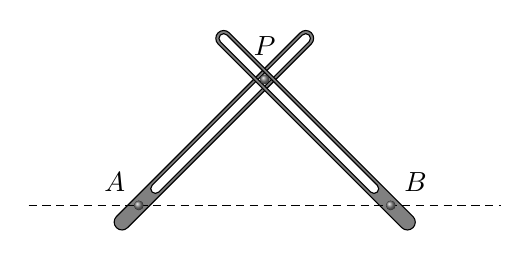
\begin{tikzpicture}[>=latex]
\begin{scope}[xshift=-1.6cm,rotate=45]
  \draw[fill=gray,even odd rule](-0.3,0.1)--(3.0,0.1)arc(90:-90:0.1)--(-0.3,-0.1)arc(270:90:0.1)(0.3,0.06)--(3.0,0.06)arc(90:-90:0.06)--(0.3,-0.06)arc(270:90:0.06);
\end{scope}
\begin{scope}[xshift=1.6cm,rotate=135]
  \draw[fill=gray,even odd rule](-0.3,0.1)--(3.0,0.1)arc(90:-90:0.1)--(-0.3,-0.1)arc(270:90:0.1)(0.3,0.06)--(3.0,0.06)arc(90:-90:0.06)--(0.3,-0.06)arc(270:90:0.06);
\end{scope}
\draw[semithick,densely dashed](-3,0)--(3,0);
\fill[ball color=gray](0,1.6)circle(0.06)node[above=5pt]{$P$};
\fill[ball color=gray](-1.6,0)circle(0.06)node[above left=2pt]{$A$};
\fill[ball color=gray](1.6,0)circle(0.06)node[above right=2pt]{$B$};
\end{tikzpicture}
\end{document}